%!TEX root = ../thesis.tex
%*******************************************************************************
%*********************************** First Chapter *****************************
%*******************************************************************************

\chapter{Results}  %Title of the First Chapter
\label{chapterresults}

\ifpdf
    \graphicspath{{Chapter5/Figs/Raster/}{Chapter5/Figs/PDF/}{Chapter5/Figs/}}
\else
    \graphicspath{{Chapter5/Figs/Vector/}{Chapter5/Figs/}}
\fi

%!TEX root = ../thesis.tex
%*******************************************************************************
%*********************************** First Chapter *****************************
%*******************************************************************************

\chapter{Results}  %Title of the First Chapter
\label{chapterresults}

\ifpdf
\graphicspath{{Chapter5/Figs/Raster/}{Chapter5/Figs/PDF/}{Chapter5/Figs/}}
\else
\graphicspath{{Chapter5/Figs/Vector/}{Chapter5/Figs/}}
\fi

One of the aims of this study was to check how the designed impedance device detects plethysmography signals. Another objective was to verify how what changes in plethysmography waveform are detectable by the instrument. As described in chapter \ref{chapterdesign} the designed device is capable of providing electrical signals comparable to the impedance of the body section. The iPG instrument provides output ports of the current driven into the patient, impedance readings and plethysmography waveform of volume under test. In chapter \ref{chapterprocedure}, these signals were converted from voltage representations into readable units such as impedance values in ohms (\si{\ohm}) and currents (\si{\ampere}. Then, a GUI provided analysis of the signals, as well as post-processing options. Last, the data was converted into measurements of blood flow.

\todo{Maybe to describe in a single line about the experimental procedure}

This chapter describes the results obtained from the experimental work. It will show the device capability of detecting impedance baseline signals and plethysmography waveforms. Later, an outline of the numeric results during occlusion will be explained when compared to the additional instruments used during the study. 

\section{Impedance baseline signal during occlusions}
\label{section5.1}
During the experimental procedure, three different level of occlusion occurred during the study. Venous blockage causes a swelling of the forearm by filling of the capillaries below the blockage. During partial arterial occlusion, the incoming arterial flow is restricted causing a slow filling of the forearm. Then, total occlusion eliminates the blood inflow under the obstructed section. 

\todo{Check about what happens during partial arterial occlusion. Slow filling of the forearm. This information should also be added to the Medical Background}

Figure \ref{fig:rb:all_participants} shows all the impedance signals of all the participants during the whole study. As can be seen, some signals were affected by motion artefact. In fact, other instruments such as PPG and ultrasound Doppler also picked up these sort of fluctuations. 

\begin{figure}
	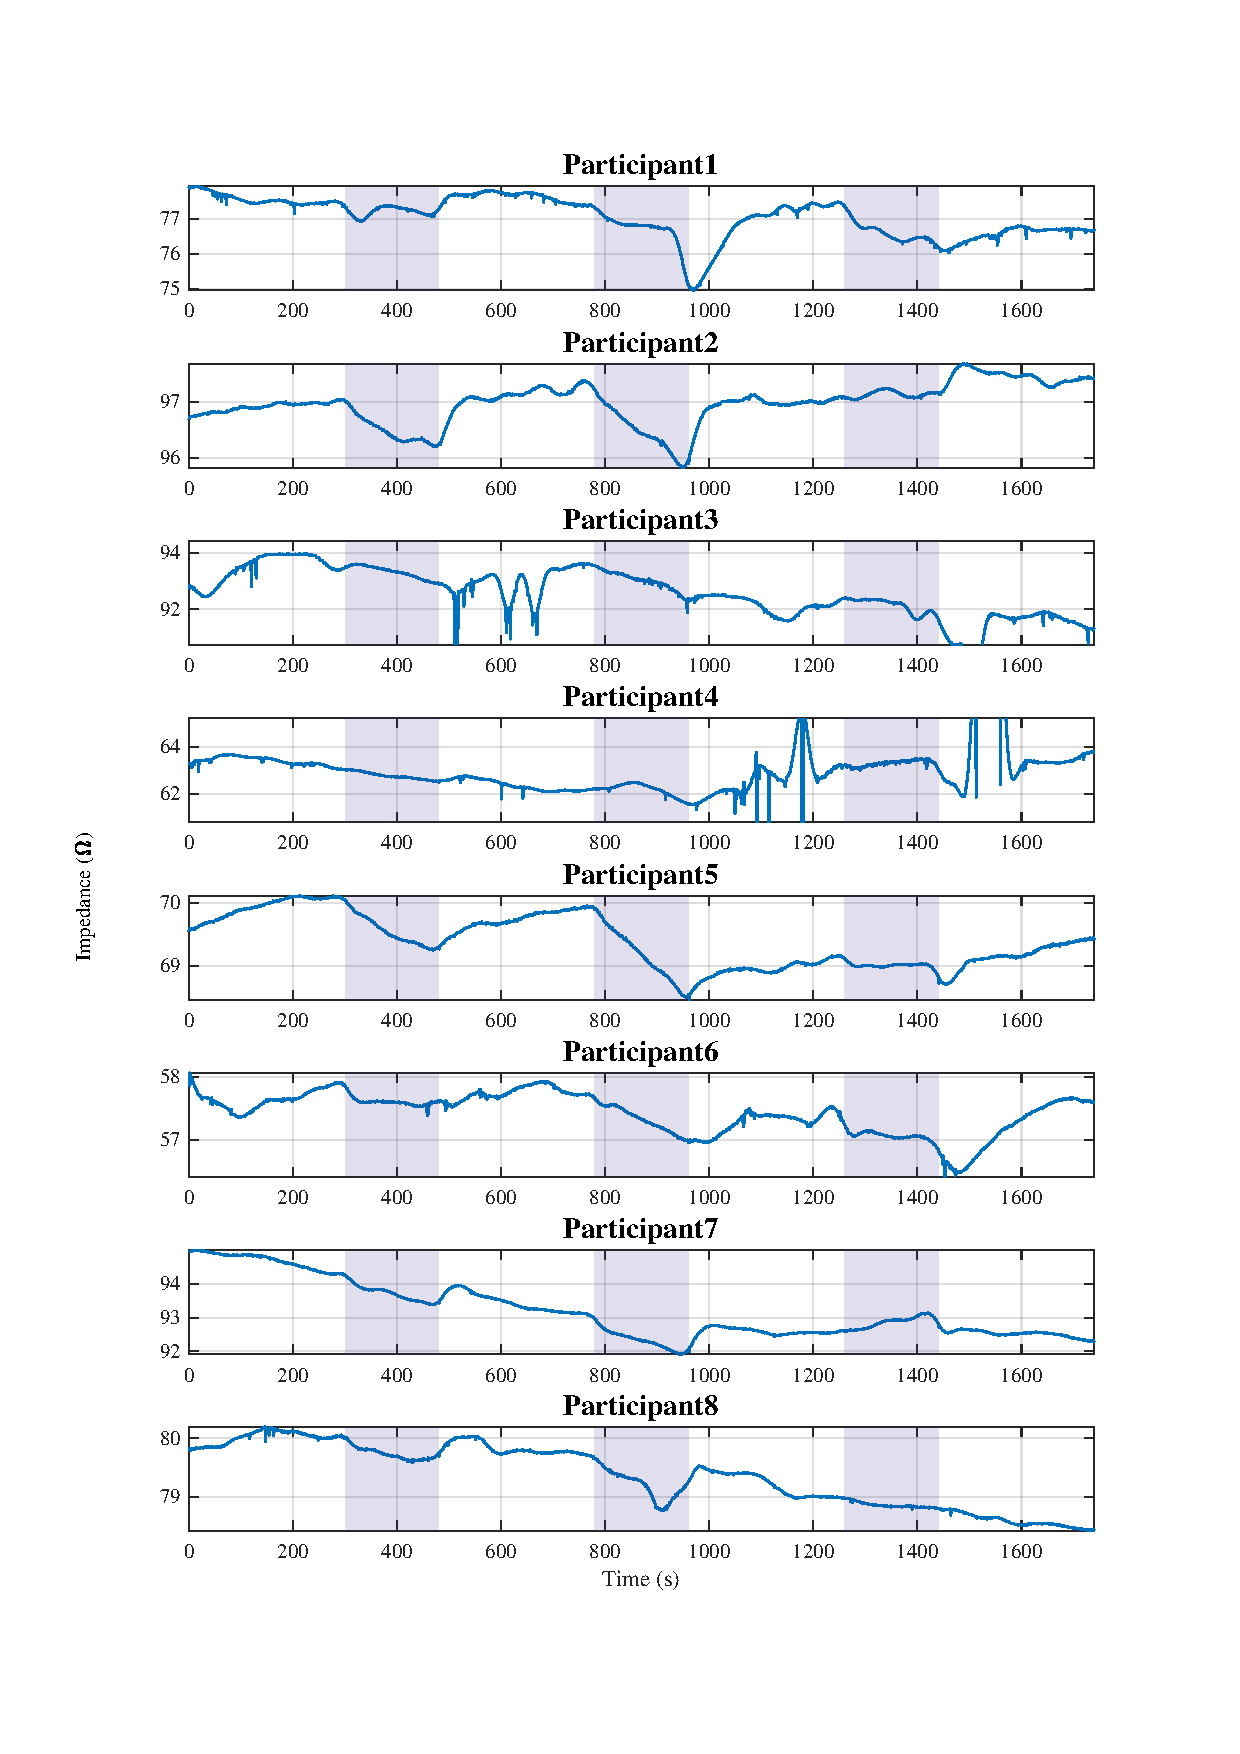
\includegraphics[width=\textwidth,height=\textheight,keepaspectratio]{figure1}    
	\caption{Baseline impedance of all the participants during the study. The shaded areas represent occlusions events.}
	\label{fig:rb:all_participants}
\end{figure}
\todo{This figure is temporary. It needs to be improved by naming axis}

\subsection{Basal impedance}
\label{section5.1.1}
The iPG device recorded the impedance during the first five minutes of data logging. As described in the previous chapters\todo{Maybe add a reference of the past chapter}, this signal is composed of the base impedance value and the AC waveform signal that is present with it. Moreover, this mean value is known as basal impedance, which it is equivalent to the value $R_B$ described by Nyober's equation \ref{eq:Nyober}. In other words, it is the value of the impedance before the circulation passes through the potential sensors. It is composed basically of the impedance contribution of bone, muscle, fat, skin and residual blood within the vessels. 

The device was able to detect the forearm's segment impedance quite remarkably. The values obtained felt within the resistive value estimated by the literature \todo{Find some papers with results about the impedance of the forearms}. The table \ref{tbl:basal_impedace:region1} describes the basal impedance during the first five minutes of data. 

\begin{table}[b]
	\caption{Basal impedance during the first five minutes of data with statistical values.}
	\label{tbl:basal_impedace:region1}
	\centering
	\begin{tabu}{ccccc}
		\hline 
		& \textbf{Mean} & \textbf{Variance} & \textbf{Maximum} & \textbf{Minimum} \\\tabucline[2pt]{-}
		Participant 1  &  \SI{77.594}{\ohm}  &   \SI{\pm0.02752}{\ohm}  &   \SI{77.374}{\ohm}  &  \SI{78.038}{\ohm}  \\
		Participant 2  &  \SI{96.968}{\ohm}  &   \SI{\pm0.00815}{\ohm}  &   \SI{96.761}{\ohm}  &  \SI{97.175}{\ohm}  \\
		Participant 3  &  \SI{93.537}{\ohm}  &   \SI{\pm0.255}{\ohm}    &   \SI{92.436}{\ohm}  &  \SI{94.063}{\ohm}  \\
		Participant 4  &  \SI{63.437}{\ohm}  &   \SI{\pm0.03548}{\ohm}  &   \SI{63.021}{\ohm}  &  \SI{63.765}{\ohm}  \\
		Participant 5  &  \SI{69.974}{\ohm}  &   \SI{\pm0.02730}{\ohm}  &   \SI{69.562}{\ohm}  &  \SI{70.198}{\ohm}  \\
		Participant 6  &  \SI{57.684}{\ohm}  &   \SI{\pm0.02798}{\ohm}  &   \SI{57.334}{\ohm}  &  \SI{58.206}{\ohm}  \\
		Participant 7  &  \SI{94.719}{\ohm}  &   \SI{\pm0.05637}{\ohm}  &   \SI{94.270}{\ohm}  &  \SI{95.053}{\ohm}  \\
		Participant 8  &  \SI{80.038}{\ohm}  &   \SI{\pm0.01250}{\ohm}  &   \SI{79.824}{\ohm}  &  \SI{80.303}{\ohm}  \\
		\hline 
	\end{tabu} 
\end{table}    

There are different aspects of the geometry that could affect the impedance reading. There have been several studies where has been demonstrated how the distance between electrodes affects readings \todo{Add reference to studies impedance vs. length}. In the current study showed that impedance was influenced by the forearm's circumference, as well as the distance between the potential electrodes. Figure \ref{fig:C_vs_Z} indicates that there is an inverse relation between circumference and impedance. The smallest the forearm's circumference higher the resistivity. On the other hand, there is a direct relation between the distance between the potential electrodes and the resistivity of the segment as depicted in \ref{fig:l_vs_Z}.

\begin{figure*}[t!]
	\centering
	\begin{subfigure}[t]{0.5\textwidth}
		\centering
		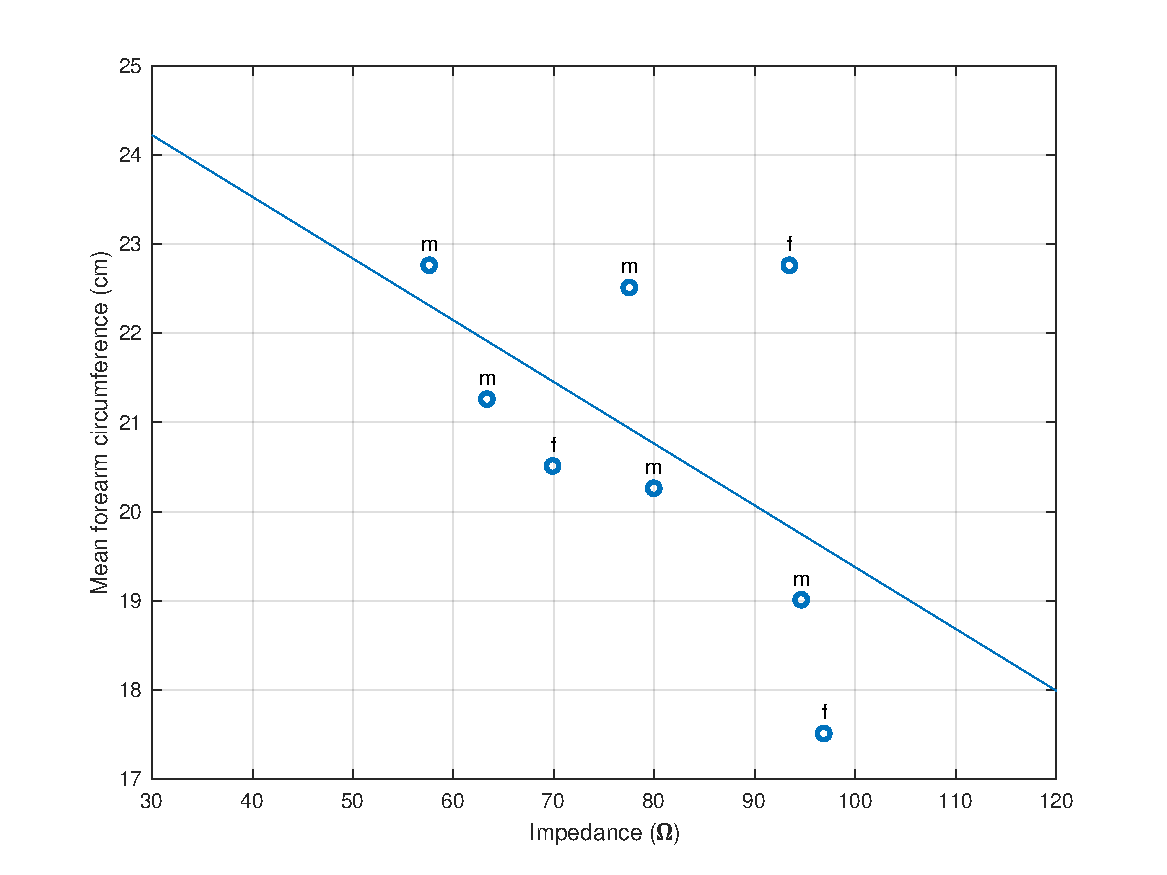
\includegraphics[height=4.5cm]{figure2a}
		\caption{Relation forearm circumference against basal impedance}
		\label{fig:C_vs_Z}
	\end{subfigure}%
	~ 
	\begin{subfigure}[t]{0.5\textwidth}
		\centering
		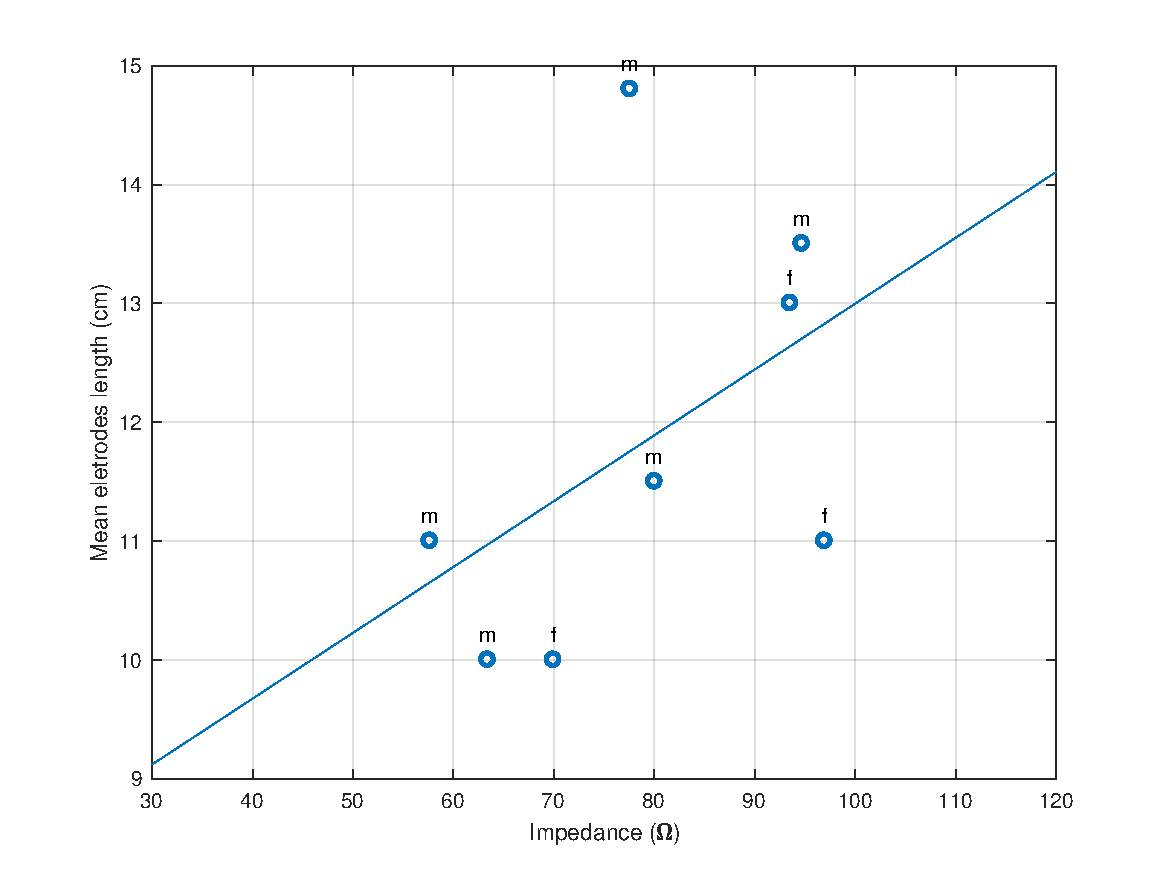
\includegraphics[height=4.5cm]{figure2b}
		\caption{Relation distance sensing electrodes against basal impedance}
		\label{fig:l_vs_Z}
	\end{subfigure}
	\caption{Relation between circumference and length affects basal impedance}
	\label{fig:relation_geometry_vs_impedance}
\end{figure*}

\subsection{Impedance during venous occlusion}
\label{section5.1.2}
During the following three minutes after the impedance venous occlusion occurred. As it can be seen in figure \ref{fig:rb:all_participants} all the participants experienced a decrease in basal impedance during this time. Most of the helpers presented a linear impedance decrease trend during the occlusion. However, some of the measurements were clearly affected by motion artefact. Participants one and six are an example of this. 

In participant one, resistance fell off immediately the occlusion occurred. Nevertheless, after a minute the patron moved his arm correcting the trend. Then, impedance continued the trend again. Furthermore,  participant six also showed similar response when the arm moved. 

The following describes how the impedance behaved during the occlusion for each participant. 


